\documentclass[12pt]{article}
\usepackage{amsmath}
\usepackage{amssymb}
\usepackage{amsfonts}
\usepackage[colorlinks=true]{hyperref}
\usepackage{graphicx}

\title{Prvi Doma\'{c}i zadatak}
\author{TZS}
\date{\today}

\begin{document}
\maketitle

U izradi doma\'{c}eg zadatka se mo\v{z}ete konsultovati medjusobno i sa mnom. Svaki doma\'{c}i koji predajete, medjutim, mora biti samostalno napisan. 

\textbf{Rok za predaju ovog doma\'{c}eg zadatka je petak 18.11.2022. Prvi i drugi zadatak nose po 8 poena a tre\'{c}i 4 poena.}

\section*{Zadatak 1}

Razmatrajmo polubeskona\v{c}nu, plan-paralelnu atmosferu u kojoj funkcija izvora na nekoj, referentnoj talasnoj du\v{z}ini zavisi od opti\v{c}ke dubine kao:
\begin{equation}
S = a + b\tau + c \tau^2
\end{equation}

\begin{itemize}
    \item Re\v{s}iti jedna{v}cinu prenosa zra\v{c}enja na referentnoj talasnoj du\v{z}ini, tj. izraziti izlazni intenzitet preko konstanti $a,b,c$. Ovaj intenzitet \'{c}emo zvati $I^+$
    \item Pretpostaviti da je odnos izmedju neprozra\v{c}nost na drugim talasnim du\v{z}inama i refererentne neprozra\v{c}nosti konstantan sa dubinom pa da mo\v{z}emo da pi\v{s}emo: 
    \begin{equation}
    \tau_\lambda = r_\lambda \, \tau
    \end{equation}
    $r_\lambda$ o\v{c}igledno govori da li je atmosfera vi\v{s}e ili manje neprozra\v{c}na na datoj talasnoj du\v{z}ini nego na referentnoj talasnoj du\v{z}ini. Re\v{s}iti jedna\v{c}inu prenosa za izlazni intenzitet i dobiti $I_\lambda^+$ kao funkciju parametara $a, b, c, r_\lambda$.
    \item Pretpostavimo (va\v{z}i za relativno velike talasne du\v{z}ine) da je funkcija izvora propoprcionalna Temperaturi. Jednostavnosti radi uzmimo da je konstanta proporcionalnosti jednaka jedan. Na\'{c}i $a, b, c$ tako da je $T(\tau=1) = 6000$, $T(\tau=0.01) = 4500$, $T(\tau=0) = 8000$. 
    \item Sa izra\v{c}unatim $a,b,c$ iz prethodnog dela, nadji opsege $r_\lambda$ za koje je izlazni intenzitet na toj talasnoj du\v{z}ini manji, odnosno ve\'{c}i od $I^+$ koje smo na\v{s}li u prvom delu.
\end{itemize}

\section*{Zadatak 2}

Tipi\v{c}na temperatura u sun\v{c}evoj fotosferi je 6000K a ukupan pritisak gasa oko $10^5 {\rm dyn/cm^2}$ \v{s}to je oko 1\,Pa. Pod pretpostavkom da je fotosfera u potpunosti sa\v{c}injena od vodonika, proceni:
\begin{itemize}
    \item Koncentraciju pozitivno naelektrisanih jona vodonika (protona), i koncentraciju elektrona.
    \item Koncentraciju negativno naelektrisanih jona vodonika. Za ovaj deo mo\v{z}ete pretpostaviti da je najve\'{c}i deo atoma vodonika neutralan. Energija jonizacije H$^-$ jona je 0.75\,eV.
    \item Uporedite koncentraciju negativno naelektrisanog jona vodonika sa koncentracijama atoma vodonika ekscitovanih na $n=3$ i $n=2$.
    \item \v{S}ta nam ovo govori o va\v{z}nosti Balmerovog, odnosno Pa\v{s}enovog kontinuuma sa apsorpciju u Sun\v{c}evoj fotosferi, u odnosu na negativan jon vodonika?
\end{itemize}

\section*{Zadatak 3}

Protuberance (eng: \emph{prominences}) i filamenti su po na\v{s}em trenutnom shvatanju jedni te isti objekti (videti sliku): relativno hladne koncentracije gasa koje pod uticajem magnetnog polja ``vise'' u Sun\v{c}evoj koroni. Filamente vidimo na disku: nevidljivi su u kontinuumu, ali se vide kao tamne ``trake'' na talasnim du\v{z}inama u centru jakih spektralnih linija (npr. H$\alpha$). Protuberance, sa druge strane, se vide iznad Sun\v{c}evog ruba kao svetle formacije u centru jakih spektralnih linija. Ukoliko su posmatra\v{c}ki uslovi izuzetni, mogu se videti i u kontinuumu. Koriste\'{c}i formalizam prenosa zra\v{c}enja, objasniti razliku izmedju protuberanci i filamenata.

\begin{figure}
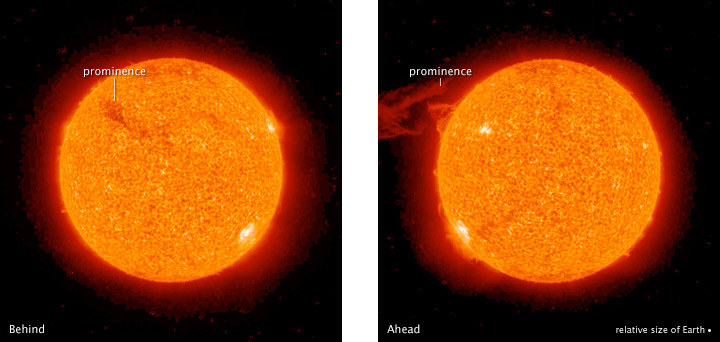
\includegraphics[width=\textwidth]{prominence.jpg}
\caption{Levo: primer sun\v{c}evog filamenta. Desno: Isti taj filament, koji se vidi kao protuberanca.}
\end{figure}




\end{document}
